% 2023
% Apéndice
% Modulación ondas electromagnéticas

\section{Introducción}
\label{sec:A92.introducción}

La transmisión y recepción de información representa uno de los logros más importantes de las telecomunicaciones, cuyas contribuciones han permitido el avance y desarrollo de un sin fin de tecnologías.

Una de las herramientas más importante de un sistema de comunicación es la \emph{modulación}.

Todas las técnicas de modulación tienen como finalidad una trasmisión más eficiente y segura de la información a través del canal utilizado como vía de enlace entre el transmisor y el receptor.

\section{Fundamentos}
\label{sec:A02.fundamentos.modulacion}

La transmisión de una señal de baja frecuencia a través del canal de un sistema de comunicación no es un proceso directo entre el transmisor y el receptor.
Para que dicha transmisión sea posible o se facilite su transmisión a través del canal del sistema, es necesario que la señal mensaje, $m(t)$,
se ajuste al rango de frecuencia en el que opera el canal de transmisión.

En los enlaces de comunicaciones las antenas receptoras utilizadas tienen como requerimiento para una adecuada recepción de la señal que sus dimensiones sean cercanas
a la décima parte de la longitud de onda de la señal recibida, $ l \sim \lambda/10$.

Por definición, la longitud de onda de una señal está dada por la siguiente expresión:

\begin{equation}
  \label{eq:A02.longitud.onda.senial} \displaystyle
  \lambda = \frac{c}{f} = \frac{3\times 10^8 \,\text{m/seg}}{f}
\end{equation}

Por ejemplo, la voz humana es una señal de baja frecuencia en el rango 300\,Hz $<$\, Voz humana \,$<$\, 3000 \,Hz, con un ancho de banda establecido en los sistemas de comunicaciones en 4 kHz.

La longitu de onda de una señal de 4 kHz es:

\[ \displaystyle
  \lambda_{4\,\text{kHz}} = \frac{ 3\times 10^8 \,\text{m/seg} }{ 4 \times 10^3\,\text{1/seg}} = 0.75 \times 10 ^5 \,\text{m} = 75000 \,\text{m}
\]

Por lo que las dimensiones de la antena necesaria para transmitir a esta frecuencia es de \textbf{\it ¡75 km!}, lo cual resulta prohibitivo para cualquier sistema.

Para subsanar este inconveniente, las señales de bajas frecuencias son trasladadas a un rango de mayor frecuencia a fin de reducir las longitudes de onda y, por lo tanto,
que las dimensiones de las antenas sean menores y de un uso práctico.

Este proceso de traslación de rango de frecuencias de una señal con información se denomina \textbf{\it Modulación}.
El mismo se logra empleando una señal portadora de mayor frecuencia que la correspondiente a la señal, $c(t)$, usualmente de forma sinusoidal, en la cual se agrega la información
a transmitir.
En la Figura \ref{fig:A02.Modulacion.senial}
se describe esquemáticamente el proceso anterior, donde puede apreciarse que el modulador mezcla la señal con la información y la señal portadora, produciendo una señal $S(t)$ modulada.

\begin{figure}[!h]
  \centering
  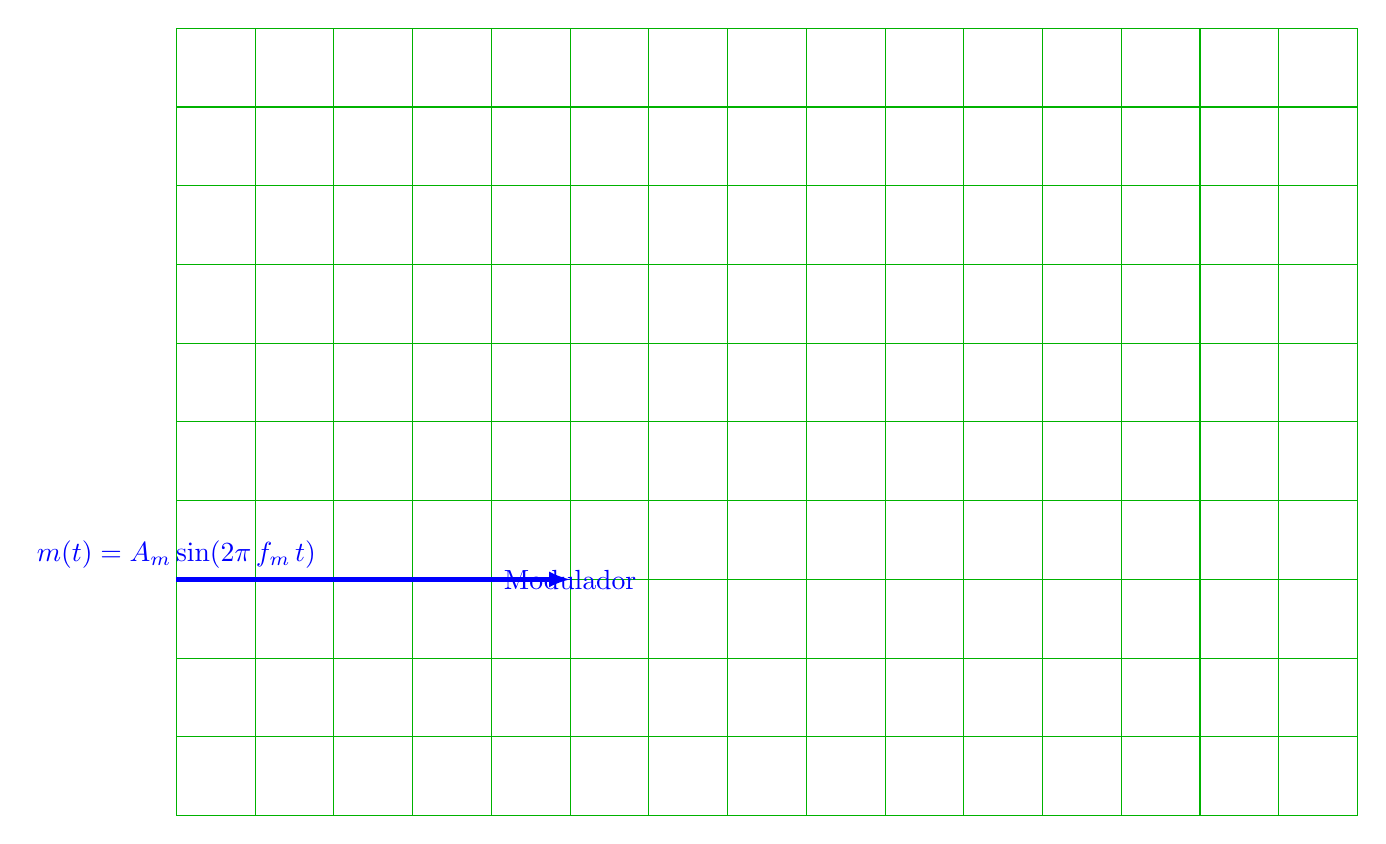
\begin{tikzpicture}[
    node distance = 2cm
    ]

    \draw [ green!70!black , step = 1 ] ( 0, 0 ) grid ( 15 , 10 ) ;

    \draw [ blue , ultra thick , -latex ] ( 0 , 3 ) node[above]  { $ m(t) = A_m \sin ( 2\pi\,f_m\,t )$}
          -- ++( 5 , 0 ) node {Modulador} 
    ;
    
%    \node (SenialInformacion) at ( 0 , 3 ) { $ m(t) = A_m \sin ( 2\pi\,f_m\,t )$} ;
    
    
    
  \end{tikzpicture}
  \caption{Esquema del proceso de modulación d euna señal.}
  \label{fig:A02.Modulacion.senial}
\end{figure}



